% !TEX TS-program = xelatex
% !TEX encoding = UTF-8 Unicode
\documentclass[aspectratio=169,11pt]{beamer}

\usetheme{Madrid}
\usecolortheme{default}
\setbeamertemplate{navigation symbols}{}
\setbeamertemplate{caption}[numbered]

\usepackage{fontspec}
\setsansfont{Latin Modern Sans}
\setmainfont{Latin Modern Roman}
\setmonofont{Latin Modern Mono}
\usepackage{graphicx}
\usepackage{booktabs}
\usepackage{array}
\usepackage{tabularx}
\usepackage{amsmath}

\definecolor{accentblue}{RGB}{22,58,105}
\definecolor{accentteal}{RGB}{20,122,112}
\definecolor{accentorange}{RGB}{232,116,28}
\definecolor{softblue}{RGB}{238,246,255}
\definecolor{ink}{RGB}{25,33,45}

\setbeamercolor{title}{fg=white}
\setbeamercolor{subtitle}{fg=white}
\setbeamercolor{frametitle}{fg=white,bg=accentblue}
\setbeamercolor{structure}{fg=accentblue}
\setbeamercolor{block title}{fg=white,bg=accentblue}
\setbeamercolor{block body}{fg=ink,bg=softblue}

\newcommand{\reportclaim}[1]{%
  \vspace{0.08cm}
  {\large\bfseries\color{accentblue}#1\par}
  \vspace{0.06cm}
}

\newcommand{\smallnote}[1]{%
  \par
  \vspace{0.08cm}
  {\footnotesize\color{ink}#1\par}
}

\newcommand{\widefig}[2][0.66\textheight]{%
  \makebox[\textwidth][c]{\includegraphics[width=0.96\textwidth,height=#1,keepaspectratio]{#2}}%
}

\newcommand{\chapterdivider}[2]{%
  \begin{frame}[plain]
    \centering
    \vspace{1.2cm}
    \makebox[\textwidth][c]{%
      \begin{beamercolorbox}[wd=0.84\textwidth,rounded=true,sep=0.42cm,center]{frametitle}
        {\LARGE\bfseries #1\par}
        \vspace{0.20cm}
        {\large #2\par}
      \end{beamercolorbox}%
    }
  \end{frame}
}

\newcommand{\twopic}[4]{%
  \begin{columns}[T,totalwidth=\textwidth]
    \begin{column}{0.49\textwidth}
      \centering
      \includegraphics[width=\linewidth,height=0.58\textheight,keepaspectratio]{#1}
      \vspace{0.04cm}
      
      {\scriptsize #2}
    \end{column}
    \begin{column}{0.49\textwidth}
      \centering
      \includegraphics[width=\linewidth,height=0.58\textheight,keepaspectratio]{#3}
      \vspace{0.04cm}
      
      {\scriptsize #4}
    \end{column}
  \end{columns}
}

\title[LViT full report]{LViT trong phân đoạn ảnh y khoa}
\subtitle{Deck đầy đủ bám theo report trong manuscript}
\author[FFT]{\texorpdfstring{Lưu Huy Minh Quang -- 23127016\\Trương Quốc Cường -- 23127333}{FFT}}
\institute[HCMUS]{Nhóm FFT -- Trường Đại học Khoa học Tự nhiên, ĐHQG-HCM}
\date{}

\begin{document}

\begin{frame}[plain]
  \centering
  \vspace{0.9cm}
  \makebox[\textwidth][c]{%
    \begin{beamercolorbox}[wd=0.88\textwidth,rounded=true,sep=0.45cm,center]{frametitle}
      {\LARGE\bfseries LViT trong phân đoạn ảnh y khoa\par}
      \vspace{0.22cm}
      {\large Deck đầy đủ bám theo report trong manuscript\par}
    \end{beamercolorbox}%
  }
  \vspace{0.35cm}
  {\large Nhóm FFT\par}
  \vspace{0.12cm}
  {\large Lưu Huy Minh Quang -- 23127016\par}
  \vspace{0.12cm}
  {\large Trương Quốc Cường -- 23127333\par}
  \vspace{0.18cm}
  {\normalsize Ứng dụng xử lý ảnh và video số\par}
\end{frame}

\begin{frame}{Cách chia task làm slide}
  \begin{itemize}
    \item \textbf{Chương 1}: chia theo bối cảnh, động lực, phát biểu bài toán, dữ liệu và đóng góp.
    \item \textbf{Chương 2}: chia theo overview, các nhóm phương pháp SOTA và research gap.
    \item \textbf{Chương 3}: chia theo từng module của LViT: luồng học/suy luận, Double-U, LV Fusion, PLAM, EPI/LV loss, loss và metric.
    \item \textbf{Chương 4}: chia chi tiết nhất, tách riêng EDA, setup, baseline, cải tiến và phân tích cho QaTa-COV19 và MosMedData+.
    \item \textbf{Chương 5}: chia theo kết luận, đóng góp, hạn chế, hướng phát triển và phần mở rộng tự giám sát.
  \end{itemize}
  \smallnote{Cấu trúc deck này bám trực tiếp theo plan trong \texttt{slides/lvit\_full\_report\_slide\_plan.md}.}
\end{frame}

\begin{frame}{Mục lục}
  \tableofcontents
\end{frame}

\section{Giới thiệu}
\chapterdivider{Chương 1}{Giới thiệu}

\begin{frame}{1.1 Bối cảnh chung}
  \twopic
    {../manuscript/figures/medical_segmentation_tasks_generated.png}
    {Phân đoạn là bài toán mức điểm ảnh, khác với phân loại và phát hiện.}
    {../manuscript/figures/lvit_data_context_generated.png}
    {Bối cảnh dữ liệu của LViT là bộ ba ảnh, văn bản và mặt nạ.}
  \smallnote{Ảnh là bằng chứng thị giác chính; mặt nạ ground truth đắt đỏ; văn bản là tín hiệu ngữ nghĩa bổ trợ dễ có hơn.}
\end{frame}

\begin{frame}{1.2 Động lực nghiên cứu}
  \twopic
    {../manuscript/figures/lvit_motivation_generated.png}
    {Ba động lực chính: ảnh mơ hồ, mask đắt và văn bản lâm sàng bị bỏ phí.}
    {../manuscript/figures/clinical_text_workflow_generated.png}
    {Quy trình lâm sàng tự nhiên đã sinh ra ảnh và văn bản cho bài toán này.}
  \smallnote{Ý nghĩa khoa học là đưa ngôn ngữ vào phân đoạn mức điểm ảnh; ý nghĩa thực tiễn là tận dụng văn bản để giảm phụ thuộc vào mask chuyên gia.}
\end{frame}

\begin{frame}{1.2 Ý nghĩa khoa học và thực tiễn}
  \begin{columns}[T,totalwidth=\textwidth]
    \begin{column}{0.49\textwidth}
      \begin{block}{Ý nghĩa khoa học}
        \begin{itemize}
          \item Đưa văn bản vào một bài toán dự đoán dày đặc, không chỉ phân loại cấp ảnh.
          \item Buộc ngữ nghĩa lâm sàng phải tác động lên biểu diễn không gian của mask.
          \item Kết nối ba hướng: CNN đặc trưng cục bộ, Transformer ngữ cảnh xa và vision-language learning.
          \item Mở rộng học bán giám sát bằng cách dùng văn bản để kiểm soát pseudo-label.
        \end{itemize}
      \end{block}
    \end{column}
    \begin{column}{0.49\textwidth}
      \begin{block}{Ý nghĩa thực tiễn}
        \begin{itemize}
          \item Tận dụng dữ liệu đã có sẵn trong quy trình đọc ảnh: ảnh + báo cáo/chú thích.
          \item Giảm phụ thuộc vào mask điểm ảnh vốn đắt và mất thời gian gán.
          \item Phù hợp với bối cảnh bệnh viện: nhiều ảnh, nhiều văn bản, nhưng ít mask chuẩn.
          \item Tạo tiền đề cho phân đoạn y khoa gần hơn với dữ liệu thật trong lâm sàng.
        \end{itemize}
      \end{block}
    \end{column}
  \end{columns}
\end{frame}

\begin{frame}{1.3 Phát biểu bài toán: đầu vào, đầu ra, ground truth}
  \reportclaim{Mỗi mẫu dữ liệu được hiểu như bộ ba \((x,t,y)\).}
  \begin{itemize}
    \item \textbf{Đầu vào}: ảnh y khoa \(x\) và văn bản chú thích/ngữ cảnh \(t\).
    \item \textbf{Đầu ra}: mặt nạ dự đoán \(\hat{y}\) ở mức điểm ảnh.
    \item \textbf{Nhãn xác thực}: mặt nạ chuyên gia \(y\) khi có; khi không có, mô hình phải học thêm từ pseudo-label.
    \item \textbf{Khung công đoạn}: mã hóa ảnh, mã hóa văn bản, hợp nhất ảnh--văn bản, học ngữ cảnh bằng hybrid CNN--Transformer, kiểm soát pseudo-label, giải mã phân đoạn.
  \end{itemize}
\end{frame}

\begin{frame}{1.3 Phát biểu bài toán: vai trò của ground truth}
  \begin{block}{Ground truth là gì?}
    Mặt nạ \(y\) là nhãn xác thực ở mức điểm ảnh, quyết định vùng nào là foreground tổn thương và vùng nào là nền.
  \end{block}
  \begin{itemize}
    \item Với dữ liệu có nhãn, \(y\) được dùng để tối ưu supervised segmentation loss.
    \item Với dữ liệu chưa nhãn, hệ thống phải sinh mục tiêu tạm thời \(\tilde{y}\) và kiểm soát độ tin cậy của nó.
    \item Vì vậy, học và đánh giá phải nhất quán: cùng kích thước ảnh/mask, cùng quy ước foreground/background, cùng metric Dice và IoU.
    \item Văn bản không thay thế \(y\); văn bản chỉ đóng vai trò prior ngữ nghĩa bổ trợ cho ảnh và pseudo-label.
  \end{itemize}
\end{frame}

\begin{frame}{1.3 Dữ liệu: QaTa-COV19}
  \twopic
    {../manuscript/figures/dataset_examples_qatacov19.png}
    {Các cặp ảnh--văn bản cho thấy cấu trúc prompt khá đều theo vị trí và số vùng nhiễm.}
    {../manuscript/figures/dataset_text_eda_qatacov19.png}
    {EDA văn bản cho thấy prompt có cấu trúc mạnh, rất thuận lợi cho text-guided segmentation.}
  \smallnote{QaTa-COV19 là miền X-quang chính để đánh giá đầy đủ ở 25\%, 50\% và 100\% nhãn.}
\end{frame}

\begin{frame}{1.3 Dữ liệu: MosMedData+}
  \twopic
    {../manuscript/figures/dataset_sources_mosmeddata.png}
    {MosMedData+ là tập CT gộp từ nhiều nguồn, nên có domain shift mạnh hơn.}
    {../manuscript/figures/dataset_examples_mosmeddata.png}
    {Cặp ảnh--văn bản của CT khó hơn vì mask nhỏ và từng lát không đồng đều.}
\end{frame}

\begin{frame}{1.3 Dữ liệu: MosMedData+ và văn bản chú thích}
  \centering
  \widefig[0.68\textheight]{../manuscript/figures/dataset_text_eda_mosmeddata.png}
  \smallnote{EDA văn bản của MosMedData+ vẫn có cấu trúc, nhưng phân bố vùng và alignment văn bản--mask yếu hơn QaTa-COV19.}
\end{frame}

\begin{frame}{1.3 Dữ liệu chính và lý do chọn}
  \begin{table}
    \centering
    \scriptsize
    \begin{tabularx}{\textwidth}{@{}l >{\raggedright\arraybackslash}X >{\raggedright\arraybackslash}X >{\raggedright\arraybackslash}X@{}}
      \toprule
      Bộ dữ liệu & Miền ảnh & Ground truth & Vai trò trong report \\
      \midrule
      QaTa-COV19 & X-quang ngực & Mask tổn thương COVID-19 + văn bản có cấu trúc mạnh & Tập chính để kiểm tra 25\%, 50\%, 100\% nhãn \\
      MosMedData+ & CT ngực đa nguồn & Mask vùng nhiễm trên lát CT + văn bản chú thích & Tập mở rộng để kiểm tra chuyển miền từ X-quang sang CT \\
      \bottomrule
    \end{tabularx}
  \end{table}
  \smallnote{Hai tập này cùng thuộc bối cảnh tổn thương phổi do COVID-19, nhưng khác mạnh về modality, kích thước foreground và mức khớp văn bản--mask.}
\end{frame}

\begin{frame}{1.3 Framework chung của hệ thống}
  \centering
  \widefig[0.70\textheight]{../manuscript/figures/lvit_system_overview_generated.png}
  \smallnote{Khung tổng quan ở mức module: ảnh, văn bản và mặt nạ đi qua mã hóa, fusion, hybrid CNN--Transformer, vòng lặp pseudo-label và decoder phân đoạn.}
\end{frame}

\begin{frame}{1.3 Framework chung: các ẩn số phải tìm}
  \begin{itemize}
    \item \textbf{Mã hóa ảnh}: học bản đồ đặc trưng đa mức từ ảnh.
    \item \textbf{Mã hóa văn bản}: học token/vector văn bản phù hợp cho phân đoạn.
    \item \textbf{Fusion ảnh--văn bản}: học cách văn bản điều chỉnh biểu diễn ảnh.
    \item \textbf{Mô hình hóa cục bộ và ngữ cảnh xa}: giữ biên nhưng vẫn hiểu bối cảnh toàn ảnh.
    \item \textbf{Kiểm soát mục tiêu tạm thời}: sinh và lọc pseudo-label cho dữ liệu chưa nhãn.
    \item \textbf{Giải mã phân đoạn}: biến đặc trưng đã hợp nhất thành mask xác suất \(\hat{y}\).
  \end{itemize}
  \smallnote{Ở Chương 1, đây mới là khung bài toán chung; các module cụ thể như Double-U, LV Fusion, PLAM, EPI hay LV loss sẽ chỉ được cố định ở Chương 3.}
\end{frame}

\begin{frame}{1.3 Phần dùng pretrained và phần học từ đầu}
  \begin{columns}[T,totalwidth=\textwidth]
    \begin{column}{0.49\textwidth}
      \begin{block}{Thành phần dùng pretrained}
        \begin{itemize}
          \item Bộ mã hóa văn bản như BERT/BiomedBERT.
          \item Vai trò: cung cấp ngôn ngữ nền, embedding giàu ngữ cảnh y sinh.
          \item Không trực tiếp tạo ra năng lực khoanh vùng tổn thương.
        \end{itemize}
      \end{block}
    \end{column}
    \begin{column}{0.49\textwidth}
      \begin{block}{Thành phần học trên tập đích}
        \begin{itemize}
          \item Backbone ảnh, fusion, decoder, pseudo-label control.
          \item Vai trò: học ánh xạ từ ảnh + văn bản sang mask.
          \item Năng lực phân đoạn vẫn phải được tối ưu trên QaTa-COV19 hoặc MosMedData+.
        \end{itemize}
      \end{block}
    \end{column}
  \end{columns}
\end{frame}

\begin{frame}{1.4 Đóng góp của báo cáo}
  \begin{columns}[T,totalwidth=\textwidth]
    \begin{column}{0.56\textwidth}
      \begin{itemize}
        \item Khảo sát lại LViT theo cách tự đủ hiểu: bối cảnh, related works, phương pháp, setup và kết quả.
        \item Phân tích dữ liệu QaTa-COV19 và MosMedData+ ở mức EDA ảnh, EDA văn bản và alignment văn bản--mask.
        \item Tái hiện baseline LViT và đọc artifact thay vì chỉ chép số liệu paper.
        \item Thử nghiệm các hướng cải tiến ảnh--văn bản và semi-supervised learning, đặc biệt trên QaTa-COV19.
      \end{itemize}
    \end{column}
    \begin{column}{0.42\textwidth}
      \begin{block}{Kết quả cải tiến chính trên QaTa-COV19}
        \small
        \begin{itemize}
          \item 25\% nhãn: \(82.22 / 73.35\)
          \item 50\% nhãn: \(84.03 / 75.62\)
          \item 100\% nhãn: \(85.28 / 77.25\)
        \end{itemize}
        \vspace{0.08cm}
        \scriptsize
        Dice / IoU test tăng rõ nhất ở điều kiện ít nhãn.
      \end{block}
    \end{column}
  \end{columns}
  \smallnote{Trọng tâm học thuật vẫn là LViT; phần cải tiến được trình bày như đóng góp bổ sung để kiểm chứng và mở rộng phương pháp.}
\end{frame}

\section{Các công trình nghiên cứu liên quan}
\chapterdivider{Chương 2}{Các công trình nghiên cứu liên quan}

\begin{frame}{2.1 Bức tranh tổng quan}
  \centering
  \widefig[0.68\textheight]{../manuscript/figures/related_taxonomy_lvit.png}
  \smallnote{Related works được nhìn như bốn nhánh hội tụ vào LViT: CNN/U-Net, Transformer/hybrid, thị giác--ngôn ngữ và học bán giám sát.}
\end{frame}

\begin{frame}{2.1 Phân loại các hướng phương pháp}
  \begin{itemize}
    \item \textbf{CNN/bộ mã hóa--bộ giải mã}: mạnh ở biên, texture và chi tiết cục bộ.
    \item \textbf{Transformer/self-attention}: mạnh ở quan hệ xa và bối cảnh toàn cục.
    \item \textbf{Hybrid CNN--Transformer}: giữ chi tiết cục bộ nhưng thêm ngữ cảnh xa.
    \item \textbf{Vision-language learning}: đưa văn bản vào biểu diễn ảnh hoặc fusion đa phương thức.
    \item \textbf{Học bán giám sát/pseudo-label}: tận dụng dữ liệu chưa có mask chuyên gia.
  \end{itemize}
  \smallnote{LViT không thuộc riêng một nhánh; nó nằm ở giao điểm của cả năm hướng này.}
\end{frame}

\begin{frame}{2.1 Benchmark, độ đo và độ phức tạp}
  \begin{itemize}
    \item \textbf{Dice} và \textbf{IoU} là hai độ đo chính để đọc mức chồng lấp giữa mask dự đoán và ground truth.
    \item Precision/recall hữu ích để hiểu mô hình đang bỏ sót tổn thương hay dự đoán lan rộng.
    \item Hiệu suất không chỉ là accuracy: còn phải nhìn \textbf{FLOPs, tham số, bộ nhớ và thời gian huấn luyện/suy luận}.
    \item Khi so sánh related works, các công trình cần được đọc theo cùng nhóm tiêu chí, tránh mỗi bài dùng một cách kể hiệu suất khác nhau.
  \end{itemize}
\end{frame}

\begin{frame}{2.1 Công tác dữ liệu và challenges}
  \begin{itemize}
    \item Ground truth y khoa mang tính chủ quan nhất định vì biên tổn thương có thể mờ và phụ thuộc chuyên gia.
    \item Văn bản chú thích và mask là hai loại giám sát khác bản chất: văn bản cho ngữ nghĩa thô, mask cho không gian chi tiết.
    \item Với bài toán ảnh--văn bản, ảnh, prompt và mask phải khớp nhau theo đúng ca/lát cắt.
    \item Thách thức tăng mạnh khi chuyển miền: X-quang khác CT, foreground nhỏ và domain shift dễ làm pseudo-label sai.
  \end{itemize}
\end{frame}

\begin{frame}{2.2 Bản đồ nhanh các công trình tiêu biểu}
  \begin{table}
    \centering
    \scriptsize
    \begin{tabularx}{\textwidth}{@{}l X X X@{}}
      \toprule
      Công trình & Vai trò trong luồng & Đóng góp chính & Hạn chế \\
      \midrule
      U-Net & Mã hóa--giải mã ảnh & Chuẩn mạnh cho segmentation y khoa ít dữ liệu & Thiếu ngữ cảnh xa, không dùng văn bản \\
      TransUNet & Lai CNN--Transformer & Kết hợp biên cục bộ và context toàn cục & Vẫn đơn phương thức ảnh \\
      GLoRIA & Ảnh--báo cáo y khoa & Chứng minh văn bản giúp học biểu diễn ảnh y khoa & Chưa trực tiếp sinh mask \\
      Mean Teacher/DTC & Học bán giám sát & Tận dụng dữ liệu chưa có mask & Pseudo-label dễ nhiễu \\
      LViT & Ảnh + văn bản + SSL & Double-U, PLAM, LV Fusion, EPI/LV loss & Phụ thuộc chất lượng văn bản \\
      \bottomrule
    \end{tabularx}
  \end{table}
\end{frame}

\begin{frame}{2.3 U-Net như đại diện nhóm CNN encoder--decoder}
  \begin{block}{Nguyên lý}
    Dùng convolution để học đặc trưng cục bộ và skip connection để khôi phục biên trong bộ giải mã.
  \end{block}
  \begin{itemize}
    \item \textbf{Phương pháp}: ảnh đi qua encoder--decoder đối xứng, đặc trưng nông được nối lại vào decoder.
    \item \textbf{Dữ liệu/ground truth}: cần cặp ảnh--mask nhất quán; không khai thác văn bản.
    \item \textbf{Đóng góp}: cực mạnh ở bài toán ít nhãn, biên cơ quan rõ, cấu trúc giải phẫu ổn định.
    \item \textbf{Hạn chế}: thiếu ngữ cảnh xa và không có cơ chế dùng thông tin ngoài ảnh.
  \end{itemize}
\end{frame}

\begin{frame}{2.4 TransUNet như đại diện hướng lai CNN--Transformer}
  \begin{block}{Nguyên lý}
    Kết hợp bản đồ đặc trưng của CNN với self-attention của Transformer để vừa giữ chi tiết cục bộ vừa học bối cảnh xa.
  \end{block}
  \begin{itemize}
    \item \textbf{Phương pháp}: CNN trích đặc trưng nền, Transformer học quan hệ giữa các token ảnh, decoder tái tạo mask.
    \item \textbf{Hiệu suất}: mở rộng tốt hơn U-Net khi tổn thương cần nhìn trong toàn cơ quan.
    \item \textbf{Đóng góp}: tạo ra cây cầu trực tiếp từ feature-based CNN sang token-based Transformer.
    \item \textbf{Hạn chế}: vẫn là mô hình ảnh-only, chưa đưa văn bản vào pipeline phân đoạn.
  \end{itemize}
\end{frame}

\begin{frame}{2.5 GLoRIA và dòng thị giác--ngôn ngữ}
  \begin{block}{Nguyên lý}
    Học căn chỉnh giữa ảnh y khoa và báo cáo/chú thích để tạo biểu diễn giàu ngữ nghĩa hơn.
  \end{block}
  \begin{itemize}
    \item \textbf{Phương pháp}: đưa ảnh và văn bản vào cùng không gian biểu diễn hoặc học tương tác ảnh--báo cáo.
    \item \textbf{Dữ liệu}: cần cặp ảnh--văn bản; không nhất thiết có mask phân đoạn.
    \item \textbf{Đóng góp}: chứng minh văn bản y khoa là nguồn tri thức thật, không chỉ là metadata.
    \item \textbf{Hạn chế}: phần lớn dừng ở mức biểu diễn toàn cục, chưa trực tiếp sinh mask mức điểm ảnh.
  \end{itemize}
\end{frame}

\begin{frame}{2.6 Mean Teacher/DTC và học bán giám sát bằng nhãn giả}
  \begin{block}{Nguyên lý}
    Tận dụng dữ liệu chưa nhãn bằng pseudo-label hoặc teacher--student consistency, nhưng phải kiểm soát sai số lan truyền.
  \end{block}
  \begin{itemize}
    \item \textbf{Phương pháp}: teacher tạo mục tiêu ổn định hơn; student học từ mask thật và nhãn giả.
    \item \textbf{Dữ liệu}: phù hợp khi ảnh nhiều nhưng mask ít.
    \item \textbf{Đóng góp}: mở rộng miền dữ liệu học mà không đòi hỏi mọi ảnh đều có ground truth.
    \item \textbf{Hạn chế}: nếu pseudo-label sai, mô hình có thể tự khuếch đại sai số qua nhiều vòng.
  \end{itemize}
\end{frame}

\begin{frame}{2.7 So sánh và research gap}
  \begin{table}
    \centering
    \scriptsize
    \begin{tabularx}{\textwidth}{@{}l c X X@{}}
      \toprule
      Hướng/công trình & Văn bản & Điểm mạnh & Điểm còn thiếu \\
      \midrule
      U-Net & Không & Biên tốt, ổn định, mạnh khi dữ liệu ít & Thiếu ngữ cảnh xa \\
      TransUNet & Không & Có cả cục bộ và toàn cục & Chưa tận dụng văn bản \\
      GLoRIA & Có & Học được ngữ nghĩa ảnh--báo cáo & Chưa sinh mask trực tiếp \\
      Mean Teacher/DTC & Thường không & Tận dụng dữ liệu chưa nhãn & Nhãn giả dễ nhiễu \\
      LViT & Có & Kết nối ảnh, văn bản và bán giám sát & Phụ thuộc chất lượng dữ liệu/văn bản \\
      \bottomrule
    \end{tabularx}
  \end{table}
\end{frame}

\begin{frame}{2.8 Research gap và dẫn dắt sang LViT}
  \begin{itemize}
    \item Gap 1: trade-off giữa chi tiết cục bộ và ngữ cảnh xa.
    \item Gap 2: văn bản y khoa chưa được đưa đủ sâu vào phân đoạn mức điểm ảnh.
    \item Gap 3: pseudo-label có ích nhưng rất dễ sai khi mask thật ít.
    \item Gap 4: khả năng tổng quát qua miền, nhất là từ X-quang sang CT, vẫn còn hạn chế.
  \end{itemize}
  \begin{block}{Dẫn dắt}
    LViT được chọn vì nó cố gắng giải quyết đồng thời cả bốn khoảng trống: kiến trúc lai, văn bản, pseudo-label và đánh giá trên nhiều miền ảnh phổi.
  \end{block}
\end{frame}

\section{Phương pháp}
\chapterdivider{Chương 3}{Phương pháp}

\begin{frame}{3.1 Tổng quan LViT}
  \centering
  \widefig[0.72\textheight]{../manuscript/figures/lvit_original_architecture.png}
  \smallnote{Kiến trúc tổng quan của LViT: Double-U kết hợp nhánh CNN, nhánh ViT đa mức, nhánh văn bản, PLAM và decoder phân đoạn.}
\end{frame}

\begin{frame}{3.1 Vai trò của từng nhánh trong LViT}
  \begin{itemize}
    \item \textbf{Nhánh ảnh CNN}: giữ biên, texture và cấu trúc không gian cục bộ.
    \item \textbf{Nhánh ViT đa mức}: học quan hệ xa giữa các vùng ảnh dưới dạng token.
    \item \textbf{Nhánh văn bản}: biến chú thích lâm sàng thành embedding có thể tác động lên đặc trưng ảnh.
    \item \textbf{PLAM + decoder}: nhấn mạnh lại tín hiệu mức điểm ảnh và khôi phục mask cuối.
    \item \textbf{EPI/LV loss}: chỉ hoạt động ở nhánh chưa nhãn, nhằm làm pseudo-label ổn định và hợp ngữ nghĩa.
  \end{itemize}
\end{frame}

\begin{frame}{3.2 Luồng học: tách rõ ba loại tín hiệu}
  \centering
  \widefig[0.66\textheight]{../manuscript/figures/lvit_training_flow_generated.png}
  \smallnote{Trong lúc học, cần tách rõ ba tín hiệu: đầu vào luôn có là ảnh \(x\) và văn bản \(t\); ground truth \(y\) chỉ có ở tập có nhãn; còn pseudo-label \(\tilde{y}\) chỉ là mục tiêu tạm cho nhánh chưa nhãn.}
\end{frame}

\begin{frame}{3.2 Ba loại tín hiệu trong quá trình học}
  \begin{columns}[T,totalwidth=\textwidth]
    \begin{column}{0.32\textwidth}
      \begin{block}{Ảnh + văn bản}
        \begin{itemize}
          \item Luôn xuất hiện ở cả train và test.
          \item Là đầu vào thật của mô hình.
        \end{itemize}
      \end{block}
    \end{column}
    \begin{column}{0.32\textwidth}
      \begin{block}{Ground truth \(y\)}
        \begin{itemize}
          \item Chỉ có ở tập có nhãn.
          \item Dùng để tạo supervised loss.
        \end{itemize}
      \end{block}
    \end{column}
    \begin{column}{0.32\textwidth}
      \begin{block}{Pseudo-label \(\tilde{y}\)}
        \begin{itemize}
          \item Chỉ có ở tập chưa nhãn.
          \item Là nhãn tạm, phải được kiểm soát.
        \end{itemize}
      \end{block}
    \end{column}
  \end{columns}
  \smallnote{Điểm then chốt của LViT là không dùng lẫn lộn \(y\) và \(\tilde{y}\): ground truth là nhãn chuyên gia, còn pseudo-label chỉ là tín hiệu học phụ trợ.}
\end{frame}

\begin{frame}{3.2 Luồng suy luận}
  \centering
  \widefig[0.66\textheight]{../manuscript/figures/lvit_inference_flow_generated.png}
  \smallnote{Luồng suy luận chỉ còn ảnh, văn bản, xác suất và nhị phân hóa theo ngưỡng; không còn loss hay cập nhật tham số.}
\end{frame}

\begin{frame}{3.3 Double-U và Vision Transformer đa mức}
  \centering
  \widefig[0.62\textheight]{../manuscript/figures/lvit_original_architecture.png}
  \begin{itemize}
    \item CNN giữ chi tiết cục bộ và cấu trúc không gian.
    \item Vision Transformer học ngữ cảnh xa trên token nhiều mức.
    \item Double-U chính là cách phối hợp hai giả định này thay vì chọn một trong hai.
  \end{itemize}
\end{frame}

\begin{frame}{3.3 Double-U: nguyên lý và vai trò}
  \begin{block}{Nguyên lý}
    CNN dựa trên giả định cục bộ của điểm ảnh, nên mạnh ở biên và texture; self-attention của Transformer học được ngữ cảnh xa và quan hệ toàn ảnh.
  \end{block}
  \begin{itemize}
    \item \textbf{Phương pháp}: nhánh CNN trích đặc trưng đa mức, nhánh ViT nhận token ảnh ở nhiều tỉ lệ rồi trả lại biểu diễn giàu context cho decoder.
    \item \textbf{Ý nghĩa}: LViT không bỏ CNN để chạy thuần token-based, mà giữ cả hai để vừa bảo toàn biên vừa hiểu bố cục tổn thương rộng.
    \item \textbf{Điểm cần nhớ}: Double-U là câu trả lời của LViT cho gap “chi tiết cục bộ vs. ngữ cảnh xa”.
  \end{itemize}
\end{frame}

\begin{frame}{3.4 Biểu diễn văn bản và LV Fusion}
  \centering
  \widefig[0.72\textheight]{../manuscript/figures/lvit_lv_fusion_generated.png}
  \smallnote{Văn bản được token hóa, chiếu về các mức kênh phù hợp và cộng/hợp nhất vào token ảnh trước Transformer block.}
\end{frame}

\begin{frame}{3.4 LV Fusion thật sự làm gì?}
  \begin{itemize}
    \item Văn bản không được gắn ở cuối như một nhãn phụ, mà đi vào \textbf{trước khi Transformer học ngữ cảnh}.
    \item Ảnh branch giữ cấu trúc không gian; text branch cung cấp gợi ý ngữ nghĩa như bên trái/phải, số vùng và mức lan tổn thương.
    \item LV Fusion chiếu embedding văn bản về đúng số kênh/token cần thiết rồi điều chỉnh token ảnh ở nhiều mức.
    \item Vì vậy, văn bản không thay ảnh; nó chỉ \textbf{điều biến cách ảnh được biểu diễn} trước khi sinh mask.
  \end{itemize}
  \smallnote{Điểm này rất quan trọng: nếu văn bản đi vào quá muộn, nó khó ảnh hưởng đến biên và vùng nhỏ trong decoder.}
\end{frame}

\begin{frame}{3.5 PLAM}
  \centering
  \widefig[0.72\textheight]{../manuscript/figures/lvit_plam_generated.png}
  \smallnote{PLAM dùng các thống kê trung bình và cực đại theo kênh để nhấn lại thông tin mức điểm ảnh trước khi decoder phục hồi mask.}
\end{frame}

\begin{frame}{3.5 PLAM: vì sao cần thêm một attention mức điểm ảnh?}
  \begin{itemize}
    \item Transformer mạnh ở quan hệ xa, nhưng có thể làm yếu thiên kiến cục bộ cần cho biên phân đoạn.
    \item PLAM nhìn lại skip feature map theo từng vị trí pixel, dùng \textbf{mean} và \textbf{max} theo kênh để tạo bản đồ điều biến.
    \item Mean giữ xu hướng chung tại mỗi vị trí; max giữ tín hiệu nổi bật tại mỗi vị trí.
    \item Decoder vì thế nhận được skip feature đã được lọc tốt hơn, giúp phục hồi biên và vùng nhỏ ổn định hơn.
  \end{itemize}
\end{frame}

\begin{frame}{3.6 EPI và LV loss}
  \centering
  \widefig[0.72\textheight]{../manuscript/figures/lvit_epi_lv_loss_generated.png}
  \smallnote{Generator sinh pseudo-label, EPI làm mượt theo vòng lặp, LV loss dùng văn bản để kiểm soát tính nhất quán ảnh--văn bản, rồi Specialist học lại từ nhãn giả đã lọc.}
\end{frame}

\begin{frame}{3.6 Bank prior của LV loss}
  \twopic
    {../manuscript/figures/lvit_lvloss_prior_gallery_page1.png}
    {8 cặp prior đầu tiên: mỗi cặp gồm một mask quy ước và một mô tả có cấu trúc.}
    {../manuscript/figures/lvit_lvloss_prior_gallery_page2.png}
    {6 cặp còn lại; tổng cộng có 14 cặp mà tác giả LViT công bố cho LV loss.}
  \smallnote{Bank prior này mã hóa các bố cục nhiễm tiêu biểu như một bên/hai bên, số vùng nhiễm và vị trí giải phẫu tương đối.}
\end{frame}

\begin{frame}{3.6 Hai tầng cosine similarity trong LV loss}
  \begin{block}{Tầng 1: chọn prior gần nghĩa nhất}
    So văn bản mẫu hiện tại với 14 câu prior bằng cosine similarity trong không gian text embedding.
  \end{block}
  \begin{block}{Tầng 2: kiểm tra pseudo-label bằng mask prior}
    Lấy mask của prior đã chọn và so tiếp với pseudo-label hiện tại bằng cosine similarity trong không gian ảnh/mask.
  \end{block}
  \begin{itemize}
    \item \textbf{EPI} ổn định pseudo-label theo thời gian bằng EMA.
    \item \textbf{LV loss} kiểm tra pseudo-label đó có còn hợp với một cấu hình ảnh--văn bản gần nghĩa hay không.
    \item Hai cơ chế bổ sung nhau: một cái ổn định theo thời gian, một cái ràng buộc theo ngữ nghĩa.
  \end{itemize}
\end{frame}

\begin{frame}{3.7 Hàm mất mát và độ đo}
\begin{columns}[T,totalwidth=\textwidth]
    \begin{column}{0.54\textwidth}
      \begin{itemize}
        \item \textbf{Nhánh có nhãn}: weighted BCE + weighted Dice.
        \item \textbf{Nhánh chưa nhãn}: weighted BCE + weighted Dice + \(0.1\times LV\_loss\).
        \item Weighted loss được dùng vì foreground nhỏ hơn nền rất nhiều trong ảnh y khoa.
        \item Nhánh chưa nhãn vẫn dùng loss phân đoạn, nhưng mục tiêu là pseudo-label đã qua EPI.
      \end{itemize}
    \end{column}
    \begin{column}{0.44\textwidth}
      \begin{block}{Cần phân biệt}
        \small
        \begin{itemize}
          \item \textbf{Loss}: tín hiệu tối ưu tham số khi học.
          \item \textbf{Metric}: cách đọc chất lượng mask sau khi dự đoán.
        \end{itemize}
      \end{block}
    \end{column}
  \end{columns}
\end{frame}

\begin{frame}{3.7 Dice và IoU trong đánh giá phân đoạn}
  \twopic
    {../manuscript/figures/dice_iou_comparison_generated.png}
    {Dice nhấn mạnh phần chồng lấp; rất hữu ích khi foreground nhỏ.}
    {../manuscript/figures/lvit_inference_flow_generated.png}
    {Trong đánh giá, mặt nạ xác suất phải được ngưỡng hóa rồi mới so với ground truth.}
  \smallnote{IoU nghiêm khắc hơn Dice vì mẫu số là phần hợp; nếu dự đoán lan rộng hoặc bỏ sót nhiều, IoU giảm mạnh hơn.}
\end{frame}

\begin{frame}{3.7 Ý nghĩa của Chương 3}
  \begin{block}{Thông điệp chốt}
    Chương 3 không chỉ kể tên module. Nó xác định luôn:
  \end{block}
  \begin{itemize}
    \item dữ liệu đi qua hệ thống như thế nào,
    \item ground truth xuất hiện ở đâu,
    \item pseudo-label được sinh và kiểm soát ra sao,
    \item và mô hình được tối ưu/đánh giá bằng những tín hiệu nào.
  \end{itemize}
  \smallnote{Nhờ vậy, Chương 4 có thể chuyển sang cài đặt và thử nghiệm mà không bị đứt mạch học thuật.}
\end{frame}

\section{Cài đặt và thử nghiệm}
\chapterdivider{Chương 4}{Cài đặt và thử nghiệm}

\begin{frame}{4.1 Mục đích thử nghiệm}
  \begin{itemize}
    \item Mục tiêu là trả lời bốn câu hỏi: LViT có tái hiện được không, baseline mạnh đến đâu, cải tiến giúp gì, và hiệu quả có còn khi chuyển sang CT hay không.
    \item QaTaLViT phải được kiểm tra đặc biệt ở 25\% và 50\% nhãn, vì đây mới là bối cảnh thiếu mask mà LViT nhắm tới.
    \item Kết quả không chỉ dừng ở Dice/IoU cuối; report còn theo dõi learning curve, pseudo-label holdout, artifact định tính và source-level behavior.
    \item Thiết kế thực nghiệm luôn tách theo từng bộ dữ liệu vì X-quang và CT có hành vi rất khác.
  \end{itemize}
\end{frame}

\begin{frame}{4.1 Kết quả chính cần chốt trước}
  \reportclaim{Phần thực nghiệm được đọc từ kết quả chính trước, rồi mới quay lại giải thích môi trường, dữ liệu và setup.}
  \begin{itemize}
    \item \textbf{QaTa-COV19}: QaTaLViT đạt \(82.22/73.35\), \(84.03/75.62\), \(85.28/77.25\) Dice/IoU ở 25\%, 50\%, 100\% nhãn.
    \item So với baseline LViT chạy lại, mức tăng lần lượt là \(+3.80\), \(+3.71\), \(+2.52\) Dice và \(+4.92\), \(+5.02\), \(+3.47\) IoU.
    \item \textbf{MosMedData+}: recipe cải tiến tốt nhất ở 50\% nhãn đạt \(73.84/60.31\), vượt rõ U-Net và cạnh tranh với LViT-T 50\%.
    \item Ý nghĩa: lợi ích lớn nhất xuất hiện khi nhãn ít hoặc khi cần kiểm soát pseudo-label tốt hơn.
  \end{itemize}
\end{frame}

\begin{frame}{4.2 Môi trường cài đặt}
  \begin{itemize}
    \item Các thử nghiệm chính được chạy trong notebook GPU trên \textbf{Kaggle}, chủ yếu với \textbf{NVIDIA Tesla T4 16GB}.
    \item Ảnh được chuẩn hóa về \(224\times224\); batch vật lý 4 kết hợp gradient accumulation 4 để đạt batch hiệu dụng 16.
    \item Pipeline bật \textbf{AMP mixed precision}, dùng \textbf{2 worker} đọc dữ liệu, cố định \textbf{seed 666}.
    \item Với nhánh văn bản pretrained, embedding có thể được cache trước để giảm chi phí lặp lại theo epoch.
  \end{itemize}
\end{frame}

\begin{frame}{4.2 Setup huấn luyện của LViT gốc và QaTaLViT}
\begin{columns}[T,totalwidth=\textwidth]
    \begin{column}{0.49\textwidth}
      \begin{block}{LViT gốc}
        \small
        \begin{itemize}
          \item Adam, \(lr=3\times10^{-4}\)
          \item Double-U + ViT đa mức
          \item Patch size \([16,8,4,2]\)
          \item Weighted Dice + BCE
          \item Checkpoint theo Dice validation tốt nhất
        \end{itemize}
      \end{block}
    \end{column}
    \begin{column}{0.49\textwidth}
      \begin{block}{QaTaLViT cải tiến}
        \small
        \begin{itemize}
          \item AdamW, \(lr=10^{-4}\), cosine scheduler
          \item 120 epoch, AMP, grad accumulation
          \item BiomedBERT 768 chiều, tối đa 10 units văn bản
          \item Teacher--student với EMA \(0.99\)
          \item Ablation theo nhóm: prompt, fusion, prior, pseudo-label control, augmentation
        \end{itemize}
      \end{block}
    \end{column}
  \end{columns}
  \smallnote{Slide này giúp người nghe thấy rõ: kết quả cải tiến không phải đến từ một thay đổi mơ hồ, mà từ một recipe đã khóa bằng hyperparameter cụ thể.}
\end{frame}

\begin{frame}{4.3 EDA QaTa-COV19}
  \twopic
    {../manuscript/figures/qatacov19_text_insights.png}
    {Ví dụ ảnh, mask và prompt của QaTa-COV19.}
    {../manuscript/figures/qata_mask_geometry_eda.png}
    {EDA hình học mask: diện tích foreground, tâm tổn thương, số component.}
\end{frame}

\begin{frame}{4.3 EDA QaTa-COV19: văn bản và alignment}
  \twopic
    {../manuscript/figures/dataset_text_eda_qatacov19.png}
    {EDA văn bản: bilateral/unilateral, số vùng và vị trí giải phẫu.}
    {../manuscript/figures/qata_text_mask_alignment.png}
    {Alignment prompt--mask tốt hơn, nên text-guided segmentation phát huy rõ.}
\end{frame}

\begin{frame}{4.3 EDA MosMedData+}
  \twopic
    {../manuscript/figures/dataset_sources_mosmeddata.png}
    {MosMedData+ là CT đa nguồn, nên domain shift mạnh hơn ngay từ đầu.}
    {../manuscript/figures/dataset_examples_mosmeddata.png}
    {Ví dụ ảnh, mask và prompt cho thấy foreground nhỏ và khó đều hơn QaTa.}
\end{frame}

\begin{frame}{4.3 EDA MosMedData+: hình học và alignment}
  \twopic
    {../manuscript/figures/mosmed_mask_geometry_eda.png}
    {EDA mask geometry của CT cho thấy foreground nhỏ và phân mảnh hơn.}
    {../manuscript/figures/mosmed_text_mask_alignment.png}
    {Alignment prompt--mask yếu hơn, giải thích vì sao CT khó hơn cho LViT.}
\end{frame}

\begin{frame}{4.3 Ground truth và tổ chức dữ liệu LViT}
  \begin{itemize}
    \item Mỗi mẫu được đọc theo bộ ba \((x,t,y)\): ảnh \(x\), văn bản chú thích \(t\), và mặt nạ \(y\) nếu có.
    \item Dữ liệu được tổ chức theo kiểu LViT: split riêng cho train/validation/test, ảnh và mask đi kèm bảng văn bản chú thích.
    \item \textbf{Ground truth} là mask nhị phân mức điểm ảnh do chuyên gia đánh nhãn; nó chỉ xuất hiện ở nhánh có nhãn và trong đánh giá.
    \item Với nhánh chưa nhãn, mô hình phải dùng pseudo-label; vì vậy chất lượng ground truth thật và cách chia nhãn/chưa nhãn là yếu tố trung tâm của toàn bộ Chương 4.
  \end{itemize}
\end{frame}

\begin{frame}{4.4 Quy trình thử nghiệm}
  \reportclaim{Thiết kế thực nghiệm được tách riêng theo QaTa-COV19 và MosMedData+.}
  \begin{itemize}
    \item QaTa-COV19 được chạy ở 25\%, 50\%, 100\% nhãn để kiểm tra rõ vai trò của văn bản và pseudo-label khi lượng mask thay đổi.
    \item MosMedData+ được đọc như bài kiểm tra chuyển miền sang CT, với baseline và recipe cải tiến tách rõ.
    \item Tất cả kết quả cuối cùng đều đọc bằng Dice/IoU; artifact trực quan được dùng để giải thích chênh lệch số liệu.
  \end{itemize}
  \centering
  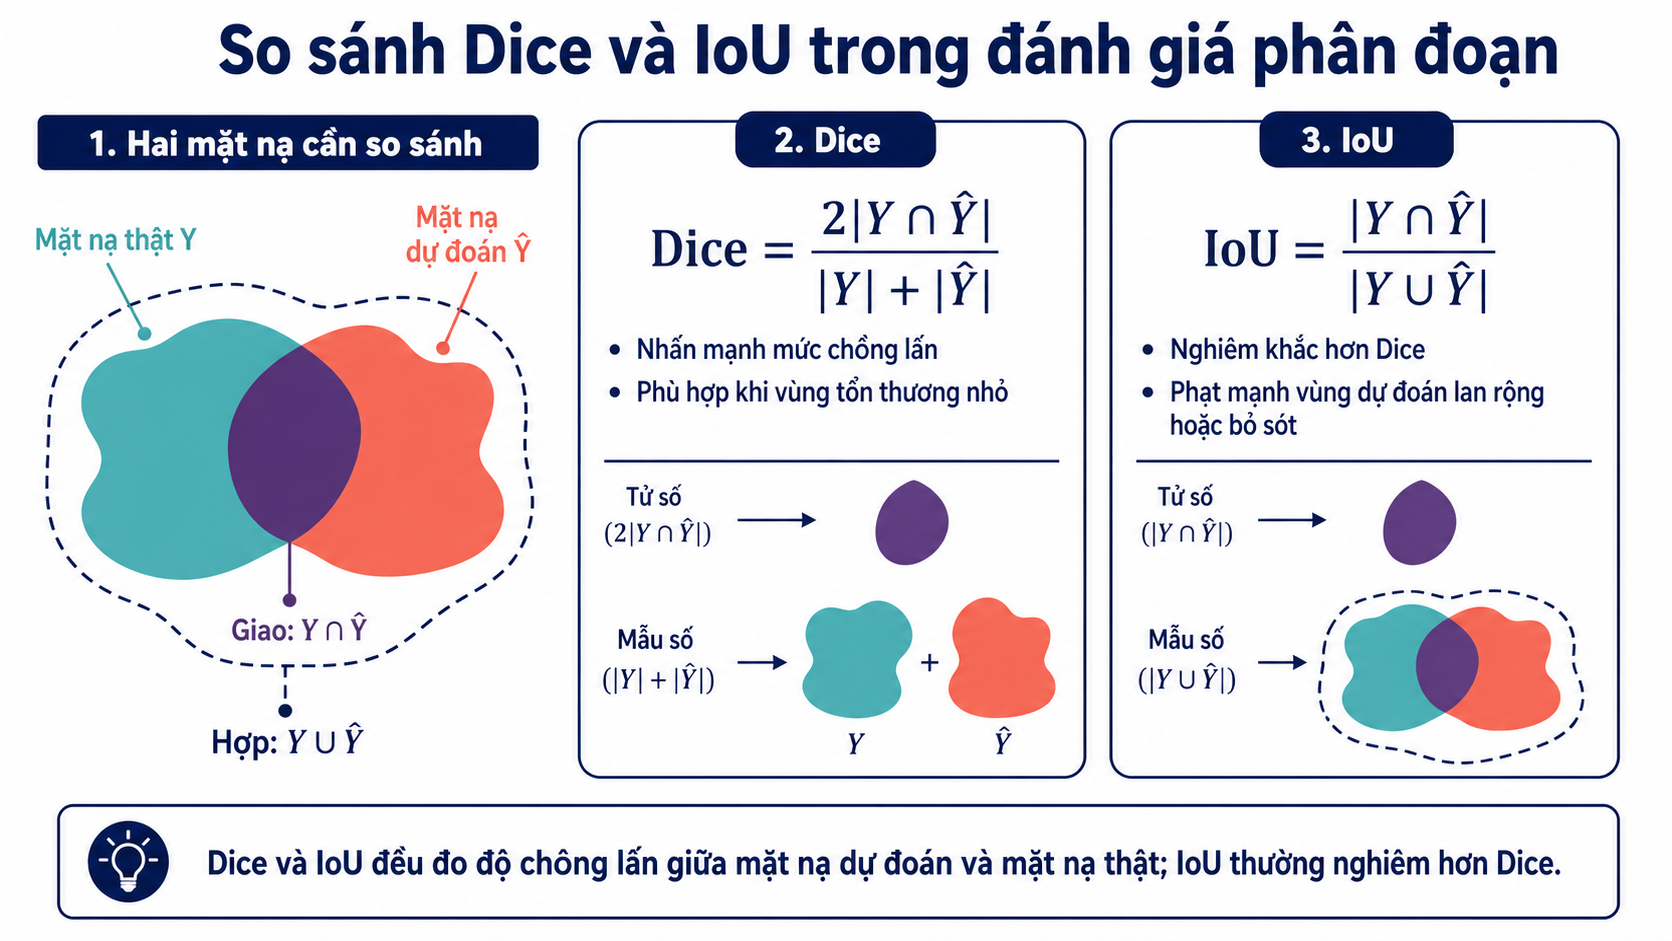
\includegraphics[width=0.54\textwidth,height=0.20\textheight,keepaspectratio]{../manuscript/figures/dice_iou_comparison_generated.png}
\end{frame}

\begin{frame}{4.4 Threshold và độ phức tạp tính toán}
\begin{columns}[T,totalwidth=\textwidth]
    \begin{column}{0.54\textwidth}
      \begin{block}{Quy ước threshold}
        \small
        \begin{itemize}
          \item \textbf{QaTa-COV19}: tất cả bảng chính dùng cố định \(\tau=0.5\).
          \item \textbf{MosMedData+}: tách rõ \textit{fixed-threshold} và \textit{validation-threshold}.
          \item Mục tiêu là tách cải thiện do mô hình khỏi cải thiện do hiệu chuẩn ngưỡng.
        \end{itemize}
      \end{block}
    \end{column}
    \begin{column}{0.44\textwidth}
      \begin{block}{Độ phức tạp tương đối}
        \small
        \begin{tabular}{lcc}
          \toprule
          Mô hình & Params & FLOPs \\
          \midrule
          LViT & 29.72M & 27.08G \\
          QaTaLViT & 25.93M & 33.67G \\
          \bottomrule
        \end{tabular}
      \end{block}
    \end{column}
  \end{columns}
  \smallnote{QaTaLViT không “nặng hơn” theo mọi nghĩa: số tham số giảm, nhưng FLOPs tăng do tương tác ảnh--văn bản và các khối phụ trợ.}
\end{frame}

\begin{frame}{4.5.1 QaTa-COV19: baseline LViT}
  \twopic
    {../manuscript/figures/lvit_baseline_25pct_training_curves.png}
    {25\% nhãn: mô hình học được tín hiệu sớm nhưng còn dao động mạnh.}
    {../manuscript/figures/lvit_baseline_50pct_training_curves.png}
    {50\% nhãn: validation Dice tăng rõ hơn nhờ nhiều mask thật hơn.}
\end{frame}

\begin{frame}{4.5.1 QaTa-COV19: tổng hợp baseline LViT}
  \begin{itemize}
    \item Khi tăng tỷ lệ nhãn từ 25\% lên 100\%, Dice và IoU cùng tăng ổn định.
    \item Mốc 50\% là điểm chuyển rõ rệt: validation bớt rung hơn và khoảng cách train--test thu hẹp.
    \item Đây là baseline để đối chiếu với công thức cải tiến QaTaLViT ở phần sau.
  \end{itemize}
  \vspace{0.15cm}
  \centering
  \small
  \begin{tabular}{lccc}
    \toprule
    Baseline LViT & 25\% & 50\% & 100\% \\
    \midrule
    Test Dice / IoU & 78.42 / 68.43 & 80.32 / 70.60 & 82.76 / 73.78 \\
    \bottomrule
  \end{tabular}
\end{frame}

\begin{frame}{4.5.1 QaTa-COV19: pseudo-label và artifact baseline}
  \twopic
    {../manuscript/figures/lvit_baseline_25pct_pseudo_holdout.png}
    {Pseudo-label 25\% có global metric khá tốt nhưng sample-level còn lệch giữa các ảnh.}
    {../manuscript/figures/lvit_baseline_50pct_pseudo_holdout.png}
    {50\% giúp pseudo-label đều hơn và bớt nhiễu hơn trên từng ảnh.}
\end{frame}

\begin{frame}{4.5.1 QaTa-COV19: artifact baseline 25\% và 50\%}
  \twopic
    {../manuscript/figures/lvit_baseline_25pct_val_artifacts.png}
    {Artifact 25\%: thường lan rộng, bỏ sót cụm nhỏ và biên chưa sắc.}
    {../manuscript/figures/lvit_baseline_50pct_val_artifacts.png}
    {Artifact 50\% tốt hơn nhưng ba kiểu lỗi chính vẫn còn.}
\end{frame}

\begin{frame}{4.5.1 QaTa-COV19: artifact baseline 100\%}
  \centering
  \widefig[0.72\textheight]{../manuscript/figures/lvit_baseline_100pct_val_artifacts.png}
  \smallnote{100\% nhãn giúp baseline mạnh hơn rõ rệt, nhưng lỗi hình thái vẫn còn: vùng dự đoán rộng, biên mờ và cụm nhỏ dễ bị nhập.}
\end{frame}

\begin{frame}{4.5.1 QaTa-COV19: kết quả cải tiến}
  \centering
  \widefig[0.58\textheight]{../manuscript/figures/qatalvit_training_artifacts.png}
  \vspace{0.05cm}
  \scriptsize
  \begin{tabular}{lccc}
    \toprule
    QaTaLViT & 25\% & 50\% & 100\% \\
    \midrule
    Test Dice / IoU & 82.22 / 73.35 & 84.03 / 75.62 & 85.28 / 77.25 \\
    \bottomrule
  \end{tabular}
  \smallnote{Độ lợi lớn nhất xuất hiện ở 25\% và 50\% nhãn, đúng với động lực ban đầu của bài toán ít nhãn.}
\end{frame}

\begin{frame}{4.5.1 QaTa-COV19: baseline vs. cải tiến}
  \centering
  \small
  \begin{tabular}{lccc}
    \toprule
    Mốc & 25\% & 50\% & 100\% \\
    \midrule
    LViT baseline & 78.42 / 68.43 & 80.32 / 70.60 & 82.76 / 73.78 \\
    QaTaLViT & 82.22 / 73.35 & 84.03 / 75.62 & 85.28 / 77.25 \\
    \midrule
    \(\Delta\) Dice & +3.80 & +3.71 & +2.52 \\
    \(\Delta\) IoU & +4.92 & +5.02 & +3.47 \\
    \bottomrule
  \end{tabular}
  \vspace{0.2cm}
  \begin{itemize}
    \item IoU tăng mạnh ở 25\% và 50\% nhãn cho thấy cải tiến không chỉ làm mask “mượt hơn”.
    \item Khi có đủ nhãn hơn, độ lợi giảm nhưng vẫn dương: văn bản và fusion vẫn hữu ích, chỉ không còn áp đảo như khi thiếu mask.
  \end{itemize}
\end{frame}

\begin{frame}{4.5.1 QaTa-COV19: pseudo-label cải tiến và so sánh}
  \twopic
    {../manuscript/figures/qatalvit_pseudo_holdout.png}
    {Pseudo-label cải tiến có chất lượng cao hơn và ổn định hơn trên phần holdout chưa nhãn.}
    {../manuscript/figures/qatacov19_training_curves.png}
    {Đường cong cải tiến trên QaTa-COV19 giữ validation ổn định hơn khi tăng tỉ lệ nhãn.}
  \smallnote{Insight chính: prompt chuẩn hóa, fusion đa mức và kiểm soát nhãn giả giúp tăng cả Dice lẫn IoU, chứ không chỉ làm mask ``mượt'' hơn.}
\end{frame}

\begin{frame}{4.5.2 MosMedData+: baseline LViT}
  \twopic
    {../manuscript/figures/mosmed_baseline_scores.png}
    {Baseline CT yếu hơn rõ so với QaTa; 25\% và 50\% còn khá sát nhau.}
    {../manuscript/figures/mosmed_baseline_training_curves.png}
    {Learning curves cho thấy convergence chậm hơn và validation trần thấp hơn.}
  \smallnote{Baseline chạy lại trên CT chủ yếu dùng để đọc hành vi pipeline và làm mốc nội bộ trước phần cải tiến.}
\end{frame}

\begin{frame}{4.5.2 MosMedData+: pseudo-label và generalization gap baseline}
  \twopic
    {../manuscript/figures/mosmed_baseline_pseudo_holdout.png}
    {Pseudo-label CT có thể đúng nhiều trên tổng pixel nhưng vẫn lệch mạnh giữa các lát.}
    {../manuscript/figures/mosmed_baseline_generalization_gap.png}
    {Generalization gap kéo dài cho thấy CT đa nguồn dễ overfit hơn X-quang.}
  \begin{itemize}
    \item Ở 50\% nhãn, baseline test chỉ đạt 59.01 / 46.11.
    \item Đây là lý do phần cải tiến trên MosMedData+ tập trung mạnh vào crop, cleanup, threshold và student-only.
  \end{itemize}
\end{frame}

\begin{frame}{4.5.2 MosMedData+: recipe cải tiến}
  \twopic
    {../manuscript/figures/mosmed_improved_scores.png}
    {Recipe cải tiến đưa kết quả CT lên rõ, đặc biệt ở 50\% nhãn.}
    {../manuscript/figures/mosmed_improved_threshold_curves.png}
    {CT rất nhạy với threshold; calibration là bắt buộc nếu muốn IoU cao hơn.}
  \vspace{0.05cm}
  \scriptsize
  \begin{tabular}{lccc}
    \toprule
    MosMed recipe & 25\% & 50\% & 100\% \\
    \midrule
    Test Dice / IoU & 65.50 / 51.32 & 73.84 / 60.31 & 73.60 / 60.12 \\
    \bottomrule
  \end{tabular}
\end{frame}

\begin{frame}{4.5.2 MosMedData+: so sánh với các mốc tham chiếu}
  \centering
  \small
  \begin{tabular}{lcc}
    \toprule
    Mốc 50\% nhãn & Dice & IoU \\
    \midrule
    U-Net & 64.60 & 50.73 \\
    LViT-T & 73.56 & 61.05 \\
    Recipe cải tiến & 73.84 & 60.31 \\
    \bottomrule
  \end{tabular}
  \vspace{0.2cm}
  \begin{itemize}
    \item So với U-Net, recipe cải tiến tăng \(+9.24\) Dice và \(+9.58\) IoU.
    \item So với LViT-T 50\%, recipe cải tiến nhỉnh \(+0.28\) Dice nhưng thấp \(-0.74\) IoU.
    \item Vì vậy, MosMedData+ nên được đọc là bài kiểm tra chuyển miền CT: kết quả cạnh tranh và giàu insight, chưa phải thắng trọn vẹn.
  \end{itemize}
\end{frame}

\begin{frame}{4.5.2 MosMedData+: artifact và source behavior}
  \twopic
    {../manuscript/figures/mosmed_improved_pseudo_holdout.png}
    {Pseudo-label cải tiến tốt hơn baseline nhưng vẫn nhạy với foreground nhỏ.}
    {../manuscript/figures/mosmed_improved_source_behavior.png}
    {Nguồn con khác nhau cho hành vi khác nhau, nên MosMedData+ phải đọc như bài kiểm tra đa nguồn.}
\end{frame}

\begin{frame}{4.5.2 MosMedData+: artifact định tính}
  \centering
  \widefig[0.68\textheight]{../manuscript/figures/mosmed_improved_val_artifacts.png}
  \smallnote{Artifact định tính cho thấy vùng rõ được bắt tốt hơn, nhưng biên mask và các cụm tổn thương nhỏ vẫn là nút thắt của miền CT.}
\end{frame}

\begin{frame}{4.5.3 Nhận xét và phân tích}
  \begin{itemize}
    \item Trên QaTa-COV19, văn bản có cấu trúc mạnh và alignment tốt với mask, nên text-guided segmentation và pseudo-label control phát huy rõ.
    \item Trên MosMedData+, bottleneck không còn chỉ là text encoder mà còn là foreground nhỏ, domain shift và threshold.
    \item Cải tiến tốt nhất không đến từ một module đơn lẻ mà từ cả recipe: prompt, fusion, pseudo-label control, crop và augmentation.
  \end{itemize}
  \begin{block}{Kết luận của Chương 4}
    LViT có thể tái hiện được như một pipeline ảnh--văn bản hoàn chỉnh; phần cải tiến làm rõ nơi nào văn bản thực sự giúp và nơi nào cần hiệu chuẩn thêm.
  \end{block}
\end{frame}

\begin{frame}{4.5.3 Kết luận chương 4}
  \reportclaim{Kết quả mạnh nhất xuất hiện đúng ở nơi bài toán khó nhất: ít nhãn trên QaTa-COV19 và chuyển miền trên MosMedData+.}
  \begin{itemize}
    \item \textbf{QaTa-COV19}: cải tiến ổn định ở cả 25\%, 50\%, 100\%; lợi nhất ở 25\% và 50\% nhãn.
    \item \textbf{MosMedData+}: văn bản vẫn hữu ích, nhưng hiệu quả phụ thuộc mạnh hơn vào crop, augmentation, threshold và source-level behavior.
    \item \textbf{Trade-off}: pipeline cải tiến có chi phí phép tính cao hơn và khó ablation hơn, nhưng đổi lại cho insight giàu hơn về text, pseudo-label và domain shift.
    \item Chương 4 vì thế không chỉ chứng minh “mô hình cao điểm số”, mà còn cho thấy \textbf{vì sao} điểm số thay đổi và \textbf{ở đâu} pipeline còn yếu.
  \end{itemize}
\end{frame}

\section{Kết luận và hướng phát triển}
\chapterdivider{Chương 5}{Kết luận và hướng phát triển}

\begin{frame}{5.1 Kết luận chung}
  \reportclaim{LViT không chỉ là một biến thể kiến trúc, mà là một cách phối hợp ba nguồn tín hiệu: ảnh, văn bản và mask chuyên gia.}
  \begin{itemize}
    \item Đầu vào gồm ảnh \(x\), văn bản chú thích \(t\), và trong giai đoạn học có thể có thêm ground truth mask \(y\).
    \item Đầu ra là mask phân đoạn \(\hat{y}\) ở mức điểm ảnh.
    \item LViT giữ CNN/Double-U cho chi tiết cục bộ, dùng Transformer cho ngữ cảnh xa, và đưa văn bản vào cả biểu diễn lẫn kiểm soát pseudo-label.
    \item Vì vậy, đóng góp chính của báo cáo không chỉ là đọc lại paper, mà là làm rõ toàn bộ chuỗi logic từ bài toán đến bằng chứng thực nghiệm.
  \end{itemize}
\end{frame}

\begin{frame}{5.2 Kết quả đạt được trên hai bộ dữ liệu}
  \begin{itemize}
    \item \textbf{QaTa-COV19}: QaTaLViT đạt \(82.22/73.35\), \(84.03/75.62\), \(85.28/77.25\) ở 25\%, 50\%, 100\% nhãn.
    \item So với baseline LViT chạy lại, mức tăng lần lượt là \(+3.80\), \(+3.71\), \(+2.52\) Dice và \(+4.92\), \(+5.02\), \(+3.47\) IoU.
    \item \textbf{MosMedData+}: recipe cải tiến tốt nhất ở 50\% nhãn đạt \(73.84/60.31\).
    \item So với U-Net \(64.60/50.73\), mức tăng là \(+9.24\) Dice và \(+9.58\) IoU; nhưng so với LViT-T 50\% \(73.56/61.05\), chỉ nhỉnh \(+0.28\) Dice và thấp \(-0.74\) IoU.
  \end{itemize}
\end{frame}

\begin{frame}{5.2 Cách đọc kết quả cho đúng}
  \begin{block}{QaTa-COV19}
    Văn bản chú thích có cấu trúc mạnh và alignment tốt với mask, nên chuẩn hóa prompt, mã hóa văn bản, fusion và pseudo-label control phát huy rõ nhất ở 25\% và 50\% nhãn.
  \end{block}
  \begin{block}{MosMedData+}
    CT đa nguồn, foreground nhỏ và prompt--mask alignment yếu hơn làm mô hình nhạy hơn với crop, augmentation và threshold; vì vậy kết quả nên được đọc là cạnh tranh và giàu insight, chưa phải thắng trọn vẹn.
  \end{block}
\end{frame}

\begin{frame}{5.3 Đóng góp của báo cáo}
  \begin{itemize}
    \item \textbf{Hệ thống hóa LViT theo khung công đoạn}: dữ liệu, mã hóa ảnh, mã hóa văn bản, fusion, mô hình hóa lai CNN--Transformer, pseudo-label control, giải mã và đánh giá.
    \item \textbf{Phân tích dữ liệu và văn bản chú thích}: chỉ ra vì sao QaTa-COV19 thân thiện hơn với text-guided segmentation, còn MosMedData+ khó hơn do CT đa nguồn và foreground nhỏ.
    \item \textbf{Tái hiện source và artifact}: không chỉ báo cáo Dice/IoU cuối mà còn có learning curves, pseudo-label holdout, threshold analysis và source-level behavior.
    \item \textbf{Kiểm tra các hướng cải tiến}: prompt normalization, BiomedBERT/NoBERT, fusion, prior/skip adapter, pseudo-label control, crop và augmentation.
  \end{itemize}
\end{frame}

\begin{frame}{5.4 Hạn chế}
  \begin{itemize}
    \item \textbf{Phụ thuộc vào chất lượng văn bản}: LViT hoạt động tốt nhất khi prompt ngắn, có cấu trúc và thật sự khớp vùng tổn thương.
    \item \textbf{Pipeline cải tiến phức tạp hơn}: số tham số giảm nhưng FLOPs tăng; chi phí chính nằm ở phép tính và độ khó vận hành, không chỉ ở kích thước mô hình.
    \item \textbf{Tổng quát qua miền còn hạn chế}: recipe tốt trên X-quang không tự động tối ưu trên CT.
    \item \textbf{Giải thích mô hình còn chưa sâu}: báo cáo đã có artifact và pseudo-label analysis, nhưng chưa đi tới attention map hay token-level explanation.
  \end{itemize}
\end{frame}

\begin{frame}{5.5 Hướng phát triển trực tiếp từ Chương 4}
  \begin{itemize}
    \item Làm chặt hơn bước xử lý văn bản: chuẩn hóa trường trái/phải, upper/middle/lower, số vùng, độ tin cậy mô tả.
    \item Làm nhẹ và làm rõ cơ chế fusion: chỉ giữ các tầng thật sự được lợi từ văn bản.
    \item Tăng độ ổn định của pseudo-label: uncertainty estimation, calibration theo validation, teacher--student consistency đa augmentation.
    \item Đánh giá cross-domain nghiêm ngặt hơn: nhiều nguồn CT/X-quang độc lập, báo cáo theo nguồn con, kích thước mask và số component.
  \end{itemize}
\end{frame}

\begin{frame}{5.6 Động lực cho hướng tự giám sát}
  \begin{itemize}
    \item Động lực không đến từ trào lưu, mà đến trực tiếp từ ba điểm nghẽn thực nghiệm:
      \begin{itemize}
        \item QaTa-COV19 còn rất nhạy với lượng mask ở 25\% và 50\%.
        \item MosMedData+ thay đổi mạnh theo nguồn CT, crop và threshold.
        \item Chất lượng pseudo-label vẫn là nút thắt nếu biểu diễn ban đầu chưa đủ tốt.
      \end{itemize}
    \item Vì vậy, tự giám sát được xem là bước \textbf{chuẩn bị biểu diễn} trước khi fine-tune bằng khung LViT, không phải thay thế LViT.
  \end{itemize}
\end{frame}

\begin{frame}{5.7 Các hướng tự giám sát sát nhất với LViT}
  \begin{itemize}
    \item \textbf{Masked image modeling}: học cấu trúc giải phẫu tổng quát trước khi có mask.
    \item \textbf{Contrastive learning trên ảnh}: đặc biệt hợp với MosMedData+ vì crop và augmentation ảnh hưởng mạnh đến kết quả.
    \item \textbf{Image--text contrastive learning}: chuẩn bị trước quan hệ ảnh--văn bản mà Chương 4 cho thấy rất hữu ích trên QaTa-COV19.
  \end{itemize}
  \begin{block}{Rủi ro cần nhớ}
    Dễ học shortcut theo nguồn ảnh, augmentation sai giải phẫu, hoặc căn chỉnh sai giữa văn bản và từng lát CT.
  \end{block}
\end{frame}

\begin{frame}{5.8 Kết luận cuối}
  \reportclaim{Trong phân đoạn ảnh y khoa, vấn đề không chỉ là có dùng văn bản hay không.}
  \begin{itemize}
    \item Văn bản chỉ hữu ích khi được chuẩn hóa đủ tốt.
    \item Văn bản chỉ phát huy khi được đưa vào đúng tầng thị giác.
    \item Pseudo-label chỉ đáng tin khi được kiểm soát theo miền dữ liệu.
    \item Vì vậy, đóng góp lớn nhất của report là làm rõ toàn bộ chuỗi logic đó trên nền LViT.
  \end{itemize}
  \begin{block}{Thông điệp chốt}
    Ảnh quyết định hình dạng mask; văn bản bổ sung ngữ cảnh; còn chất lượng cuối cùng phụ thuộc vào cách ta phối hợp và kiểm soát hai nguồn thông tin này.
  \end{block}
\end{frame}

\end{document}
